\chapter{determination of exchange stiffnessness}



\section{Measurement of ST-FMR on circular devices}


\begin{figure}[!ht]
\centering
\subfigure{\label{fig:C07MR}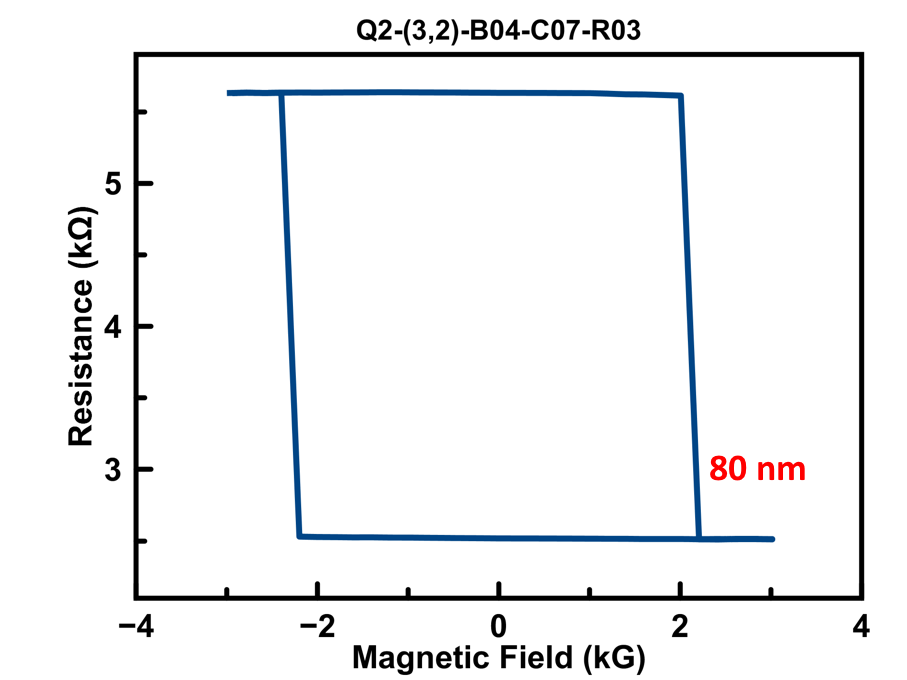
\includegraphics[width=75mm]{fig/2018/C07MR}}
\subfigure{\label{fig:C07FH}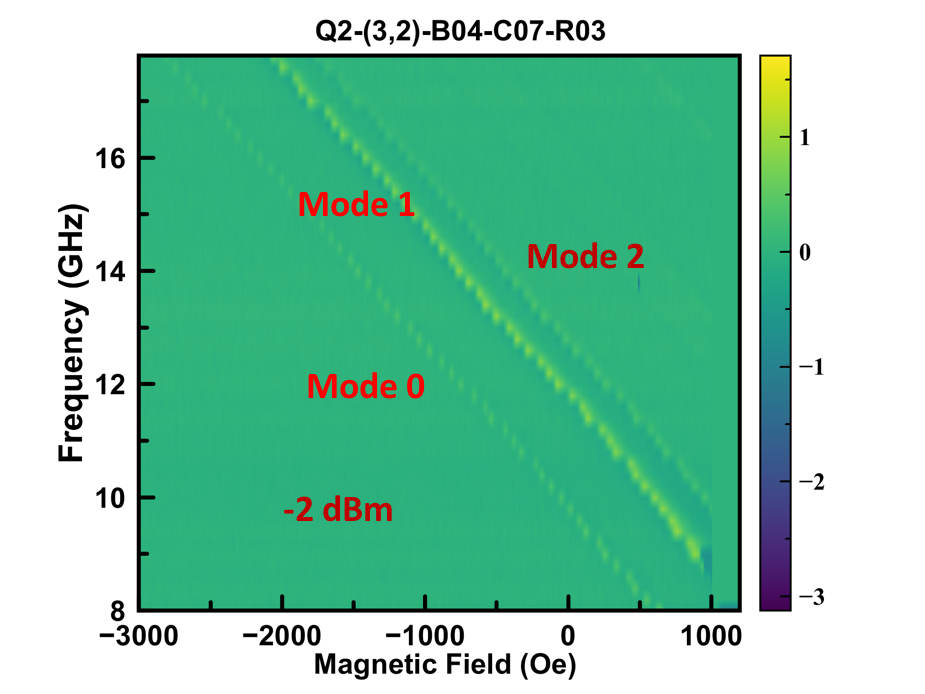
\includegraphics[width=75mm]{fig/2018/C07FH}}
\caption{}
\end{figure}




\begin{figure}[!ht]
  \centering
  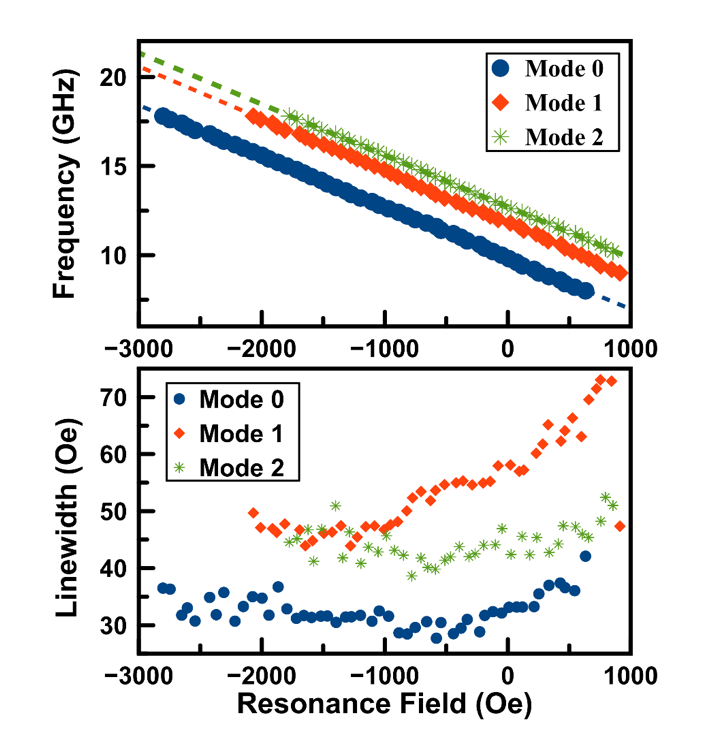
\includegraphics[width=0.6\textwidth]{fig/2018/C07fit}
   \caption{07 sample fit}
  \label{fig:07fit}
\end{figure}





\newpage



\section{Study of signal amplitude of ST-FMR signal}


\begin{figure}[!ht]
\centering
\subfigure{\label{fig:C10MR}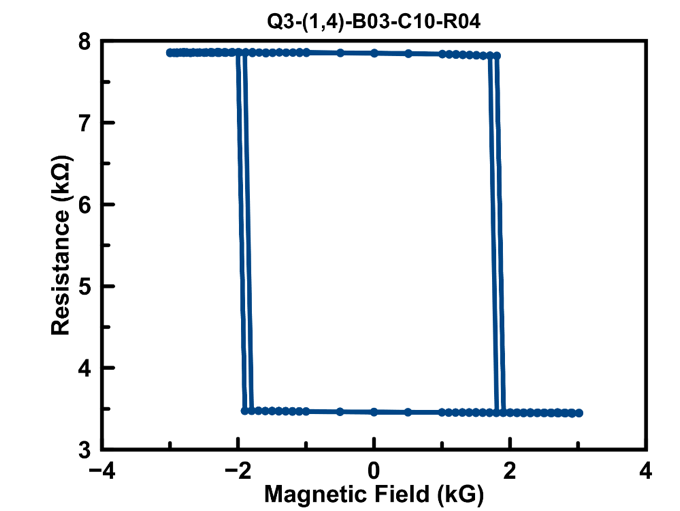
\includegraphics[width=50mm]{fig/2018/C10MR}}
\subfigure{\label{fig:C10RDC}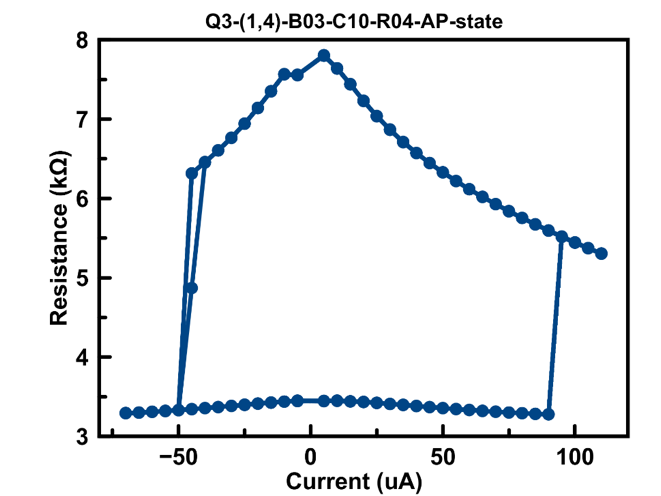
\includegraphics[width=50mm]{fig/2018/C10RDC}}
\subfigure{\label{fig:C102D}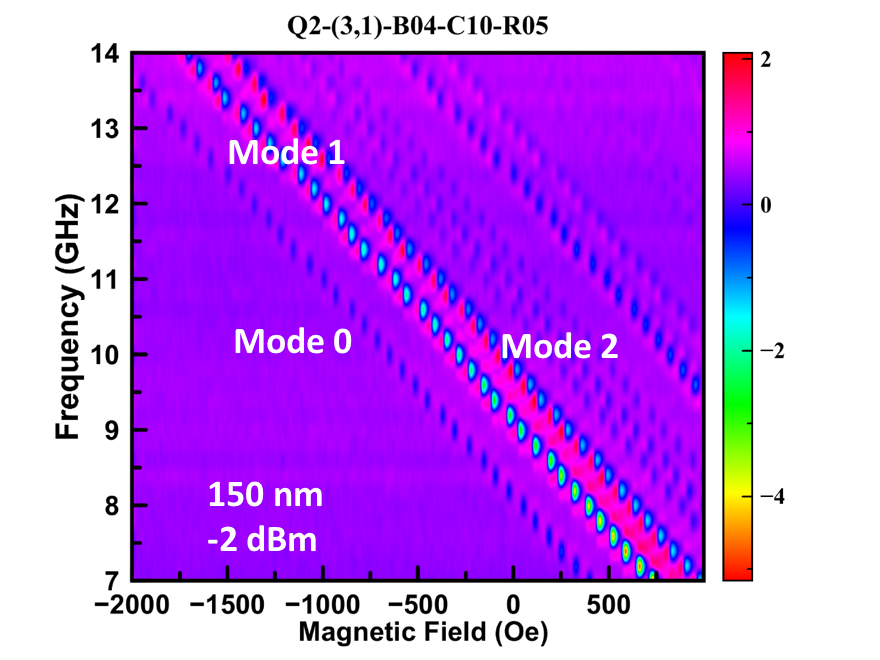
\includegraphics[width=50mm]{fig/2018/C102D}}
\caption{}
\end{figure}



\begin{figure}[!ht]
\centering
\subfigure{\label{fig:C10FH}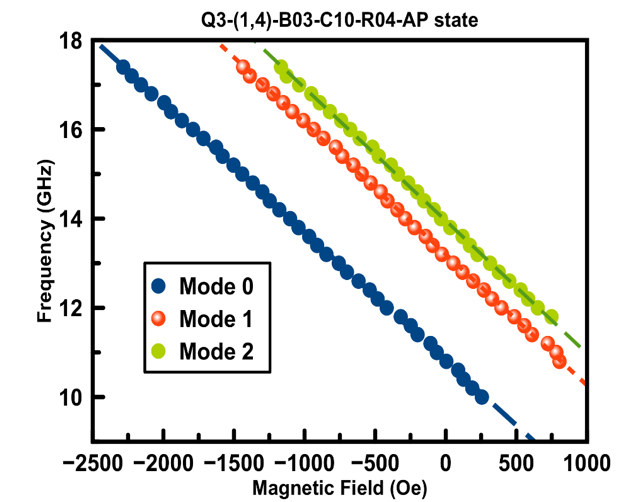
\includegraphics[width=50mm]{fig/2018/C10fit}}
\subfigure{\label{fig:C10signal}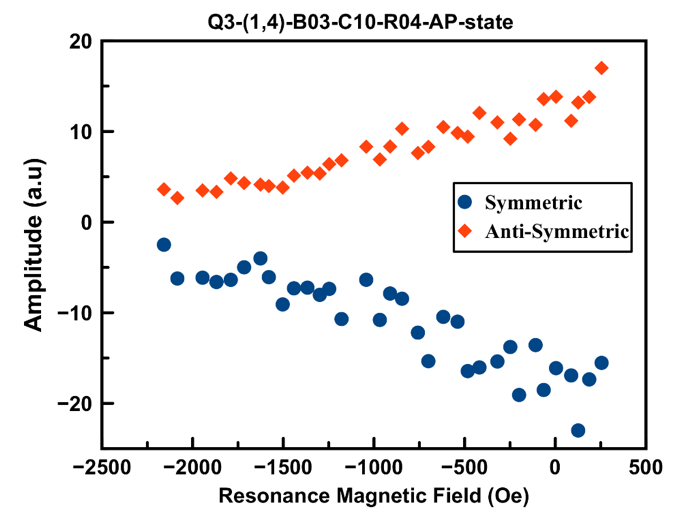
\includegraphics[width=50mm]{fig/2018/C10signal}}
\subfigure{\label{fig:C10ratio}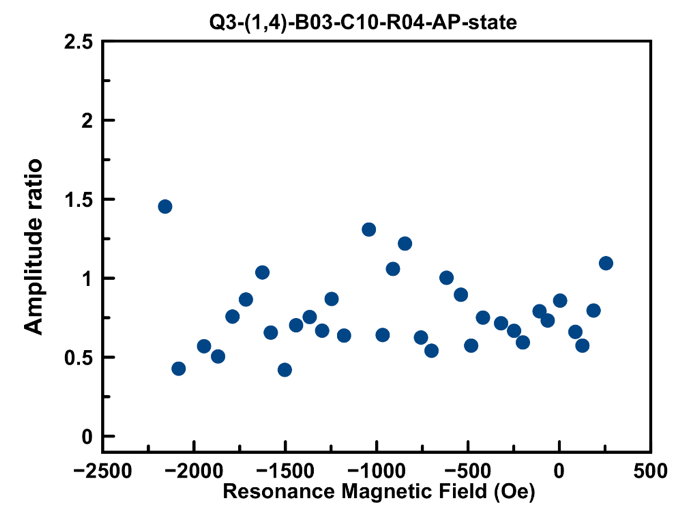
\includegraphics[width=50mm]{fig/2018/C10ratio}}
\caption{}
\end{figure}




\begin{figure}[!ht]
\centering
\subfigure{\label{fig:C10power}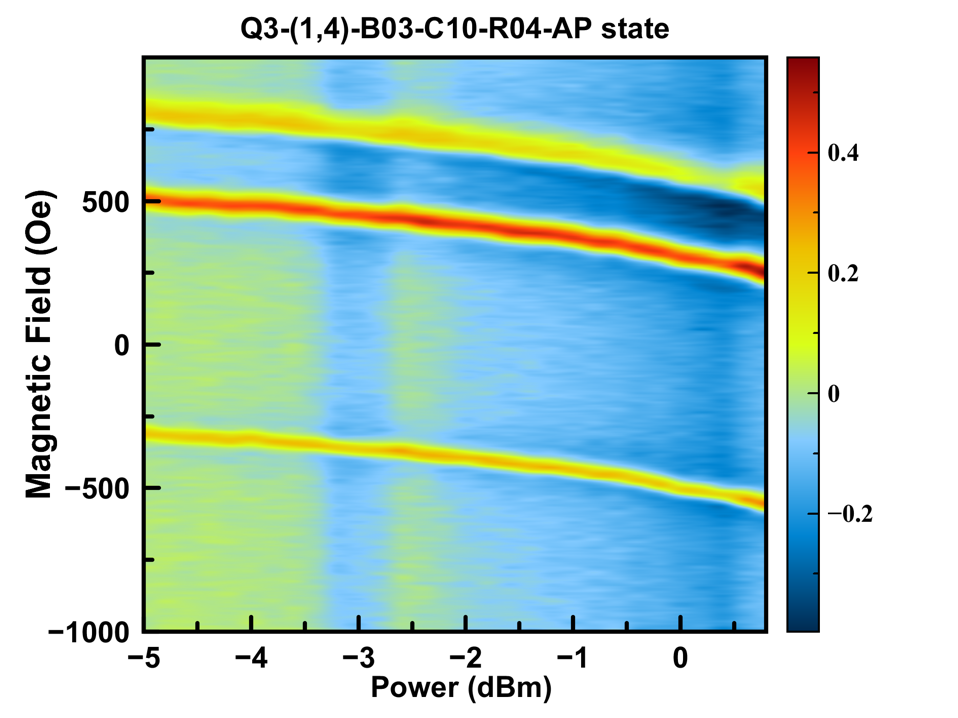
\includegraphics[width=75mm]{fig/2018/C10power}}
\subfigure{\label{fig:C10poweramp}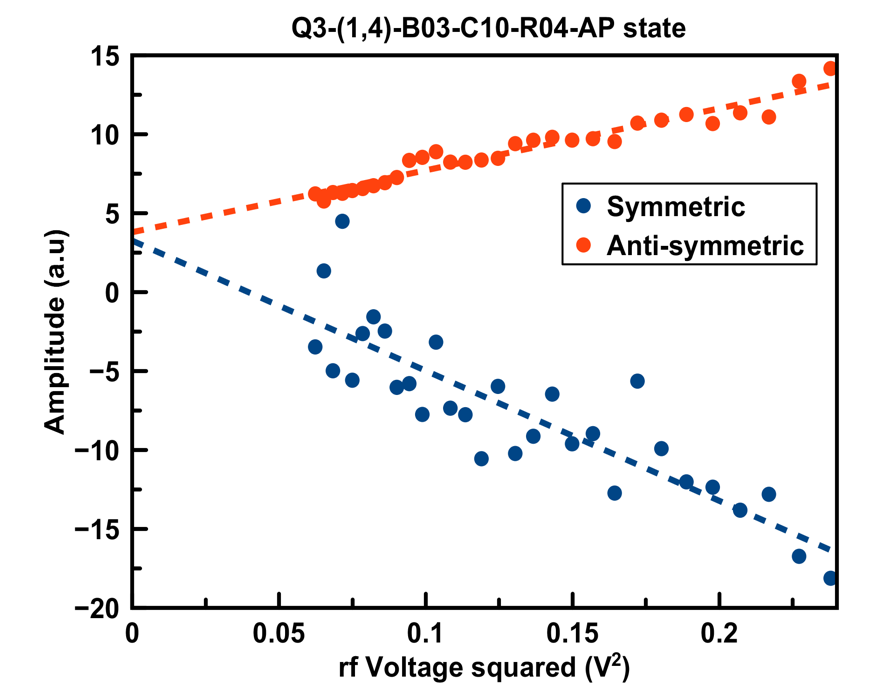
\includegraphics[width=75mm]{fig/2018/C10powersignal}}
\caption{}
\end{figure}




\begin{figure}[!ht]
\centering
\subfigure{\label{fig:C10powerfit}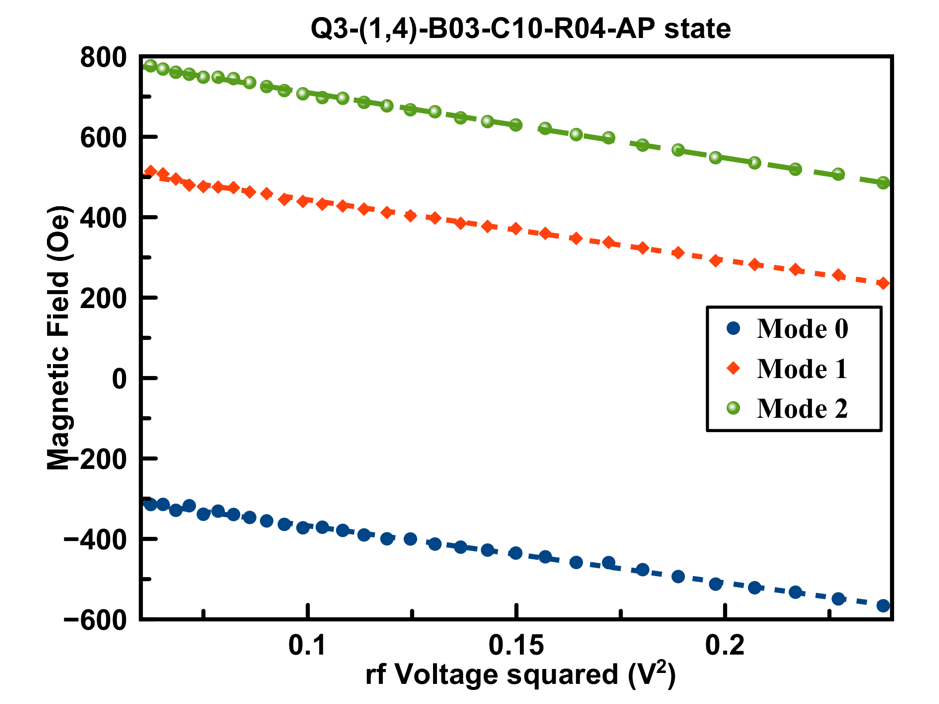
\includegraphics[width=75mm]{fig/2018/C10powerFH}}
\subfigure{\label{fig:C10powerLW}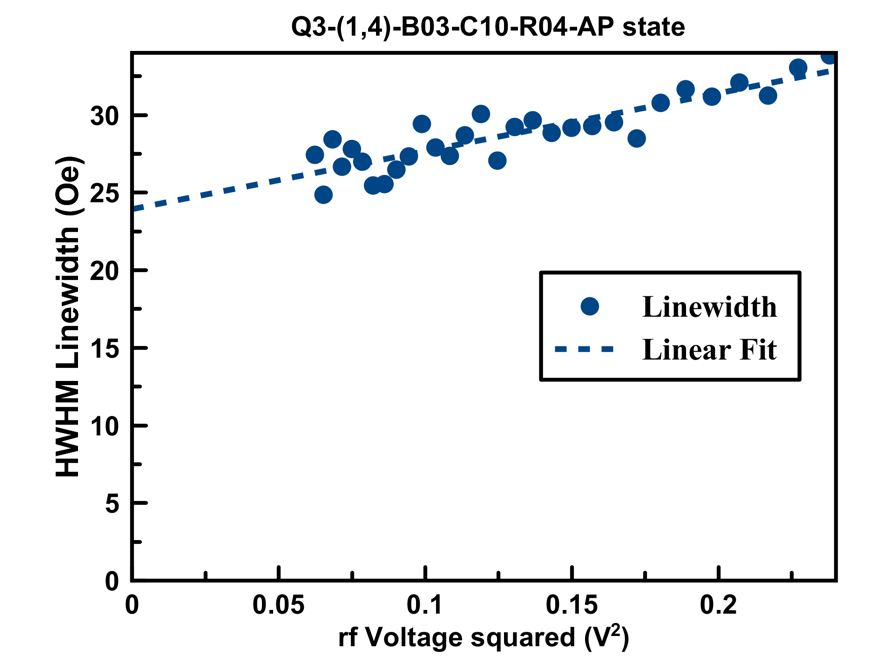
\includegraphics[width=75mm]{fig/2018/C10powerLW}}
\caption{}
\end{figure}

\begin{figure}[!ht]
\centering
\subfigure{\label{fig:C10DC}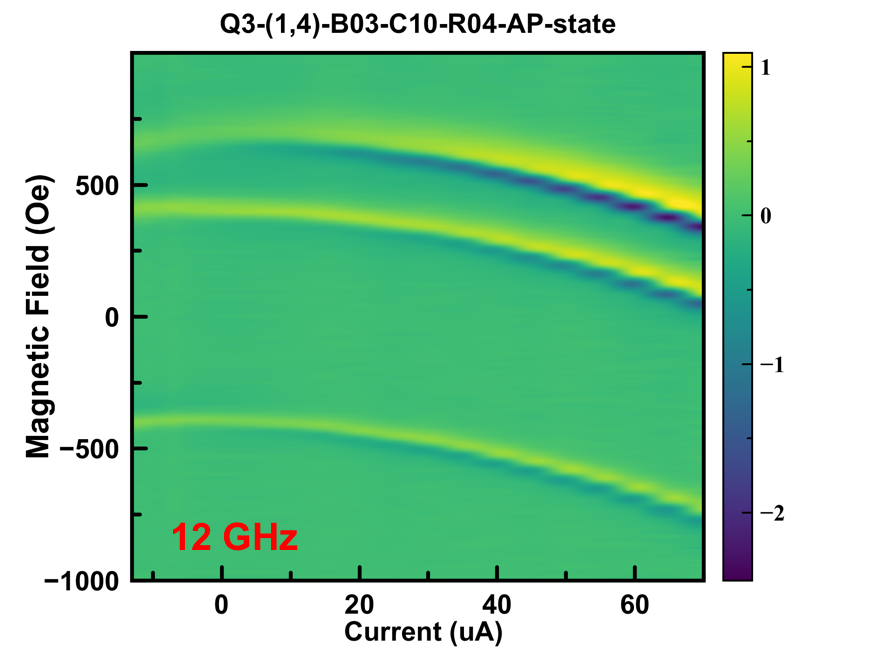
\includegraphics[width=75mm]{fig/2018/C10DC}}
\subfigure{\label{fig:C10DCamp}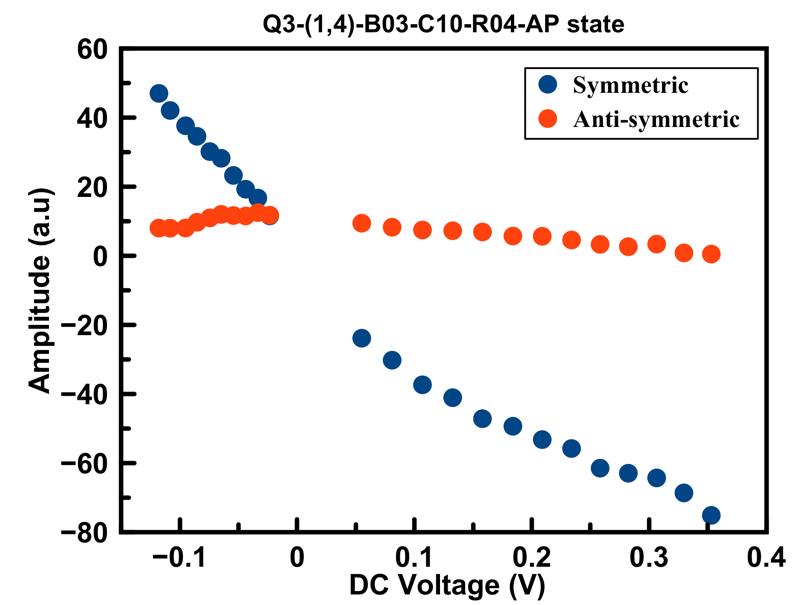
\includegraphics[width=75mm]{fig/2018/C10DCsignal}}
\caption{}
\end{figure}




\begin{figure}[!ht]
  \centering
  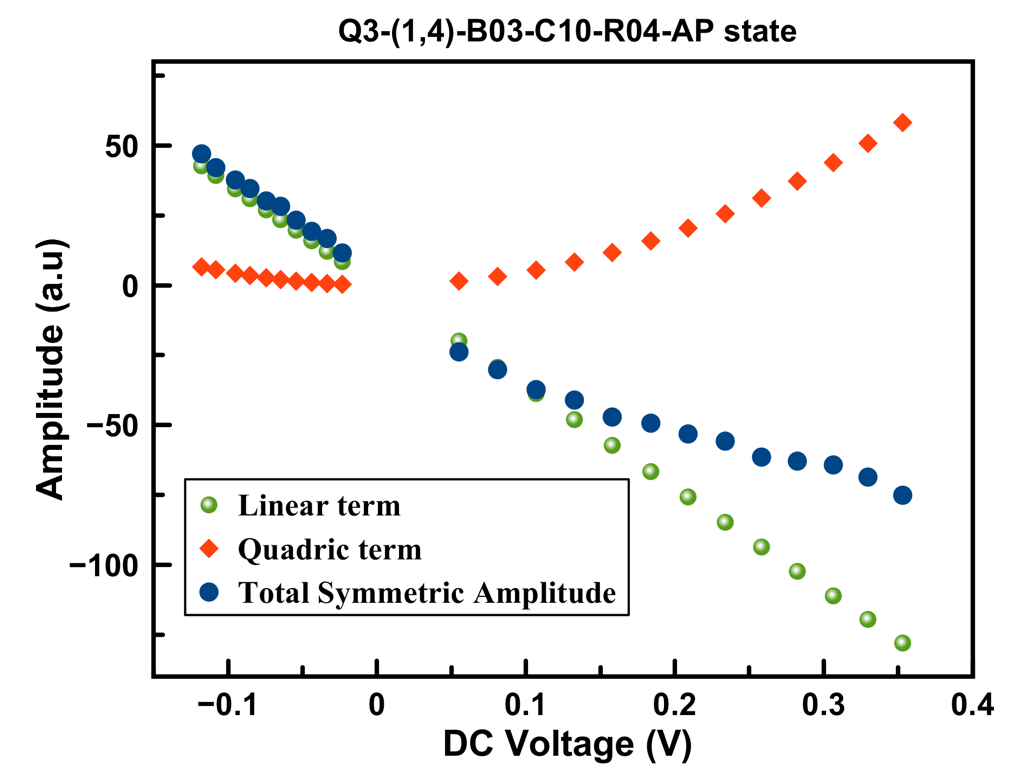
\includegraphics[width=0.8\textwidth]{fig/2018/C10DCFIT}
   \caption{C10 sample fit}
  \label{fig:C10DCfit}
\end{figure}



\begin{figure}[!ht]
\centering
\subfigure{\label{fig:C10DCFH}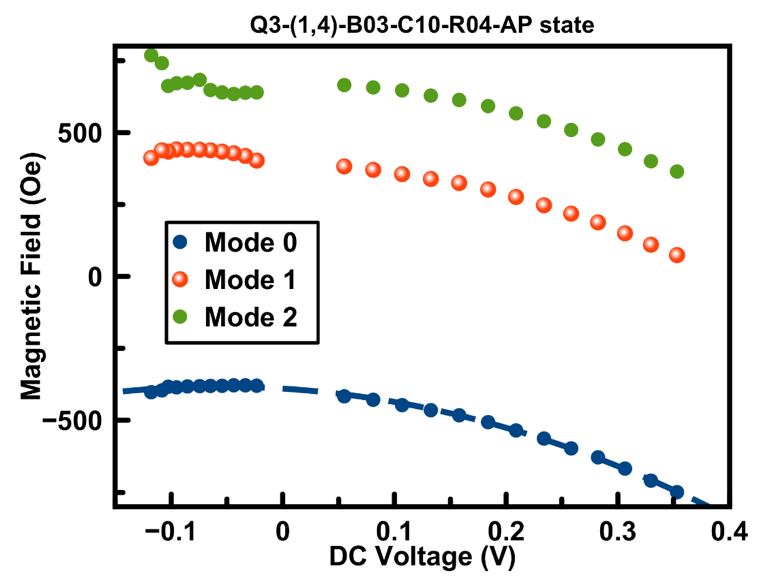
\includegraphics[width=75mm]{fig/2018/C10DC-FH}}
\subfigure{\label{fig:C10DCLW}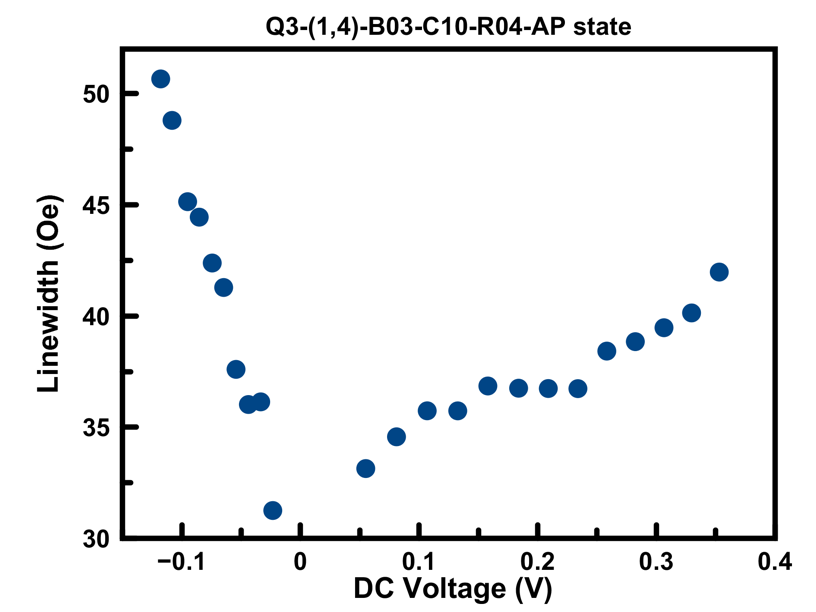
\includegraphics[width=75mm]{fig/2018/C10DC-LW}}
\caption{}
\end{figure}



\clearpage




\section{Summary of Circular Devices}



\begin{figure}[!ht]
  \centering
  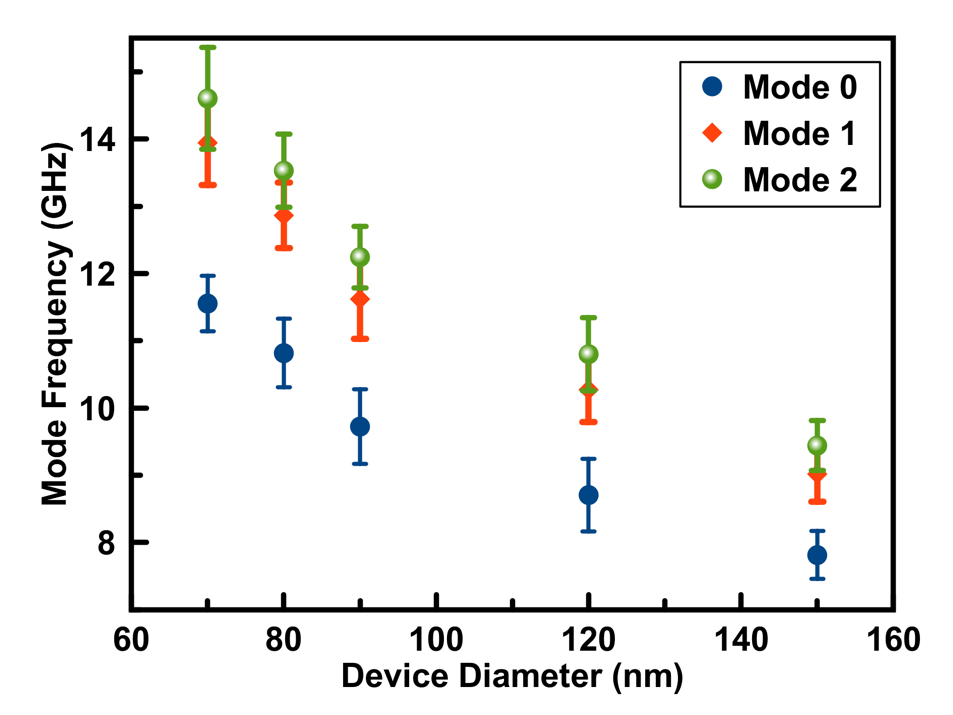
\includegraphics[width=0.6\textwidth]{fig/2018/ModevsSize}
   \caption{Mode vs Size}
  \label{fig:ModeVsSize}
\end{figure}



The effective demagnetization factor is
\begin{equation}\label{eq:Nz}
	\centering
	N_z \approx 1- \frac{1}{\pi d} [2 \ln(4 \frac{d}{t} ) -1 ]
\end{equation}

where the d is the device diameter and t is the free layer thickness. Eq.\ref{eq:Nz}

The total perpendicular anisotropy $H_ku$ can be written as 

\begin{equation}\label{eq:Hk}
	\centering
	H_k = H_{ku} + 2 \pi (1 - 3 N_z) M_s
\end{equation}

Assuming the free layer thickness 1.6 nm, the fitted result  $M_s  1820 emu/cm^3$ and  $H_{ku}$  24 KOe.



\begin{figure}[!ht]
\centering
\subfigure{\label{fig:GapvsSize}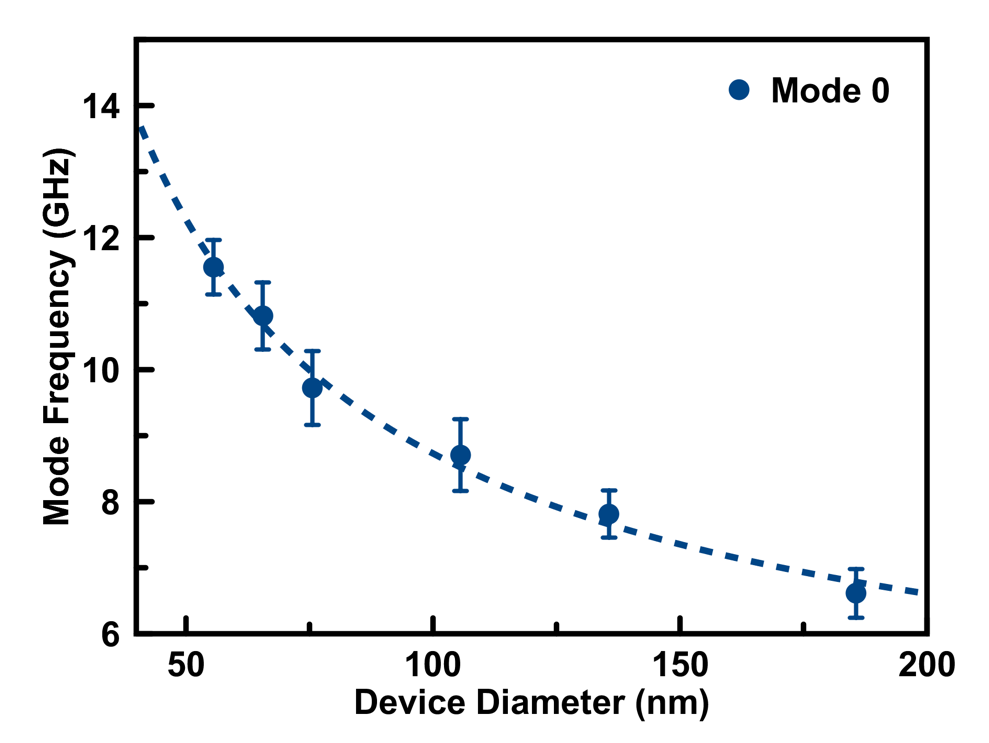
\includegraphics[width=75mm]{fig/2018/GapvsSize}}
\subfigure{\label{fig:LinearFit}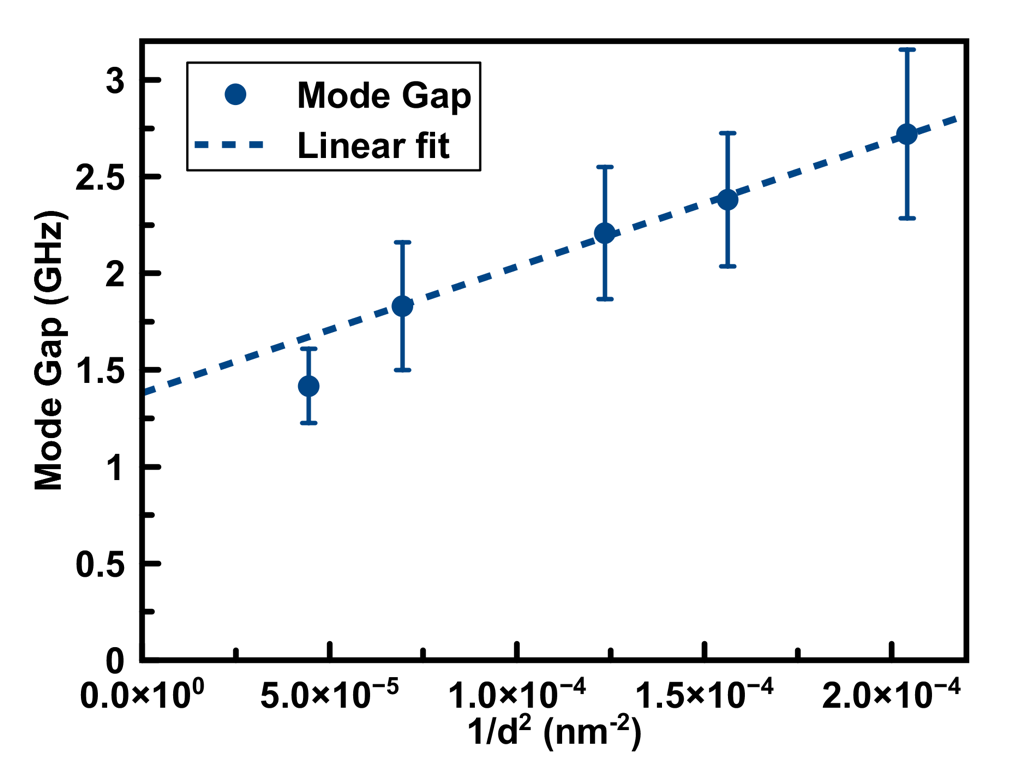
\includegraphics[width=75mm]{fig/2018/LinearFit}}
\caption{}
\end{figure}


\clearpage


\section{Micromagnetic Simulations of the Mode Spacing}

\begin{figure}[!ht]
  \centering
  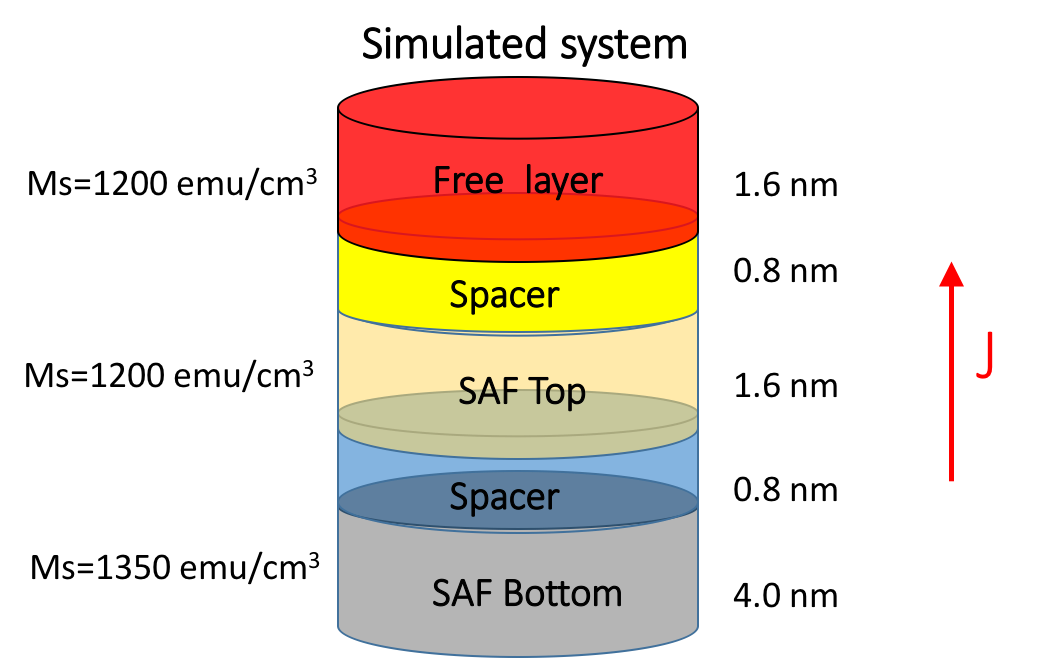
\includegraphics[width=0.8\textwidth]{fig/2018/simulated}
   \caption{Simulated MTJ System}
  \label{fig:simulated}
\end{figure}



Used parameter $ A_ex  12 pJ/m $
$ K_u 10.5*105 J/m^3$


\begin{figure}[!ht]
\centering
\subfigure{\label{fig:7070}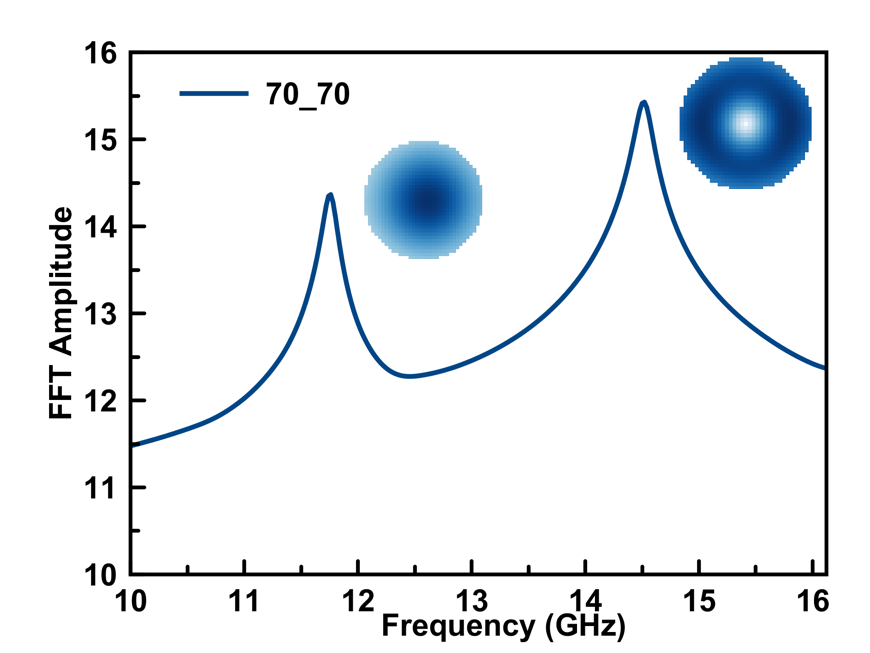
\includegraphics[width=50mm]{fig/2018/sim/70_70}}
\subfigure{\label{fig:ellipse}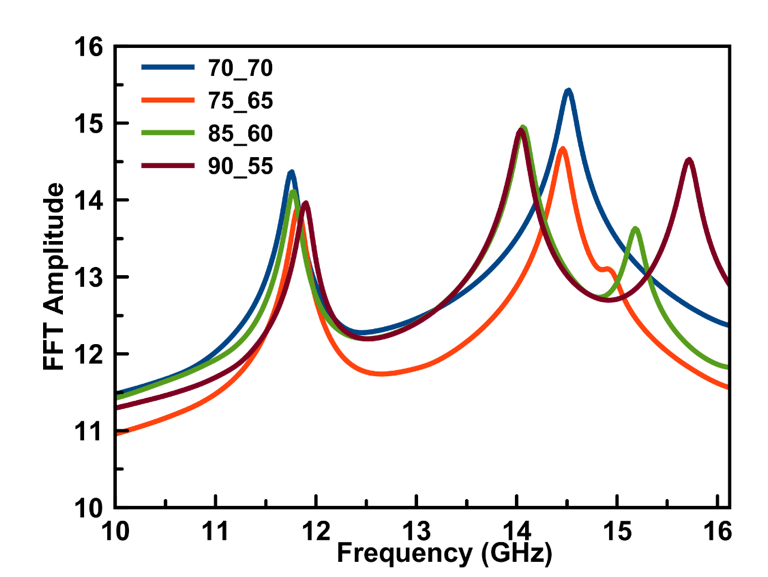
\includegraphics[width=50mm]{fig/2018/sim/ellipse}}
\subfigure{\label{fig:shape}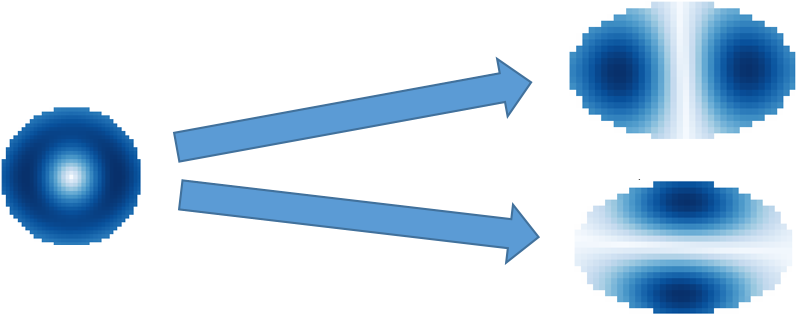
\includegraphics[width=50mm]{fig/2018/sim/split}}
\caption{}
\end{figure}



\begin{table}[ht!]
\centering
\begin{tabular}{|l|l|l|l|l|l|}
\hline
\textbf{} & \textbf{70*70} & \textbf{75*65} & \textbf{85*60} & \textbf{90*55} & \textbf{Experimental} \\ \hline
\textbf{Mode 0} & 11.74 & 11.82 & 11.78 & 11.9 & 11.55 \\ \hline
\textbf{Mode 1} & 14.5 & 14.46 & 14.06 & 14.04 & 13.94 \\ \hline
\textbf{Mode 2} &  & 14.9 & 15.2 & 15.72 & 14.6 \\ \hline
\textbf{Gap (1+2)/2-0} & 2.76 & 2.86 & 2.85 & 2.9 & 2.72 \\ \hline
\textbf{Gap 2-1} & 0 & 0.44 & 1.14 & 1.68 & 0.66 \\ \hline
\textbf{Aspect ratio} & 1 & 1.15 & 1.41 & 1.63 &  \\ \hline
\end{tabular}
\caption{Shape distortion}
\label{shapedist}
\end{table}


\begin{figure}[!ht]
  \centering
  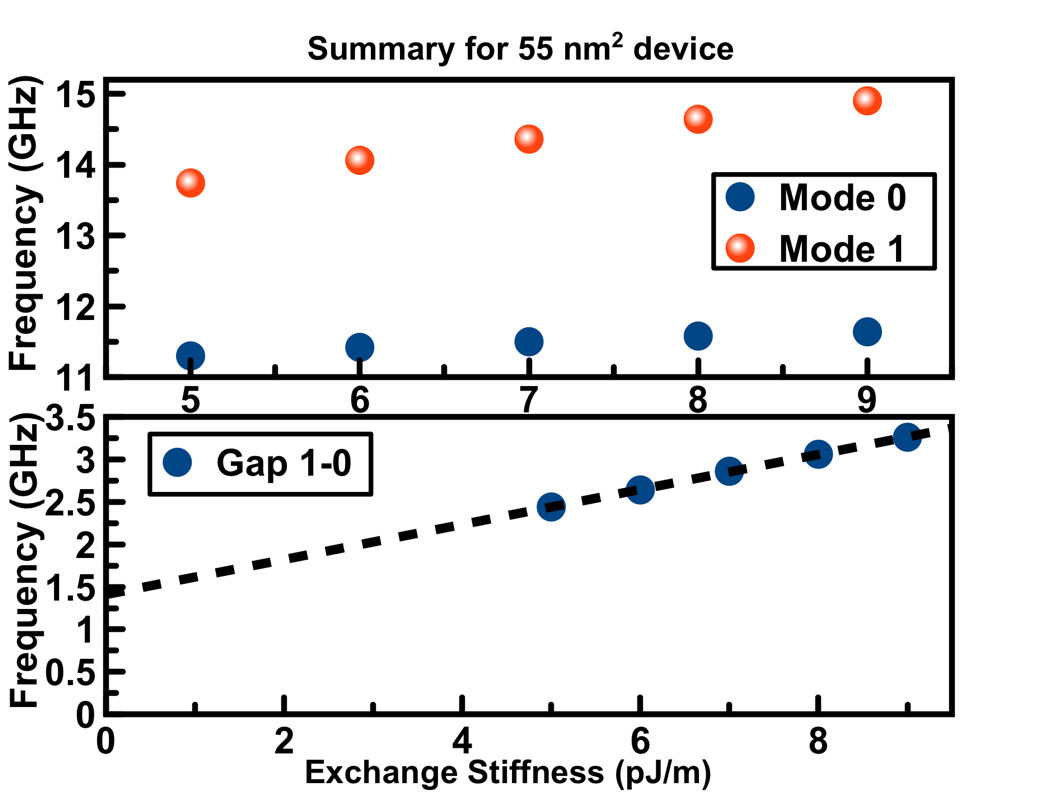
\includegraphics[width=0.8\textwidth]{fig/2018/sim/55sim}
   \caption{55 simulated}
  \label{fig:55sim}
\end{figure}



\begin{table}[ht!]
\centering
\begin{tabular}{ c c }
      \addheight{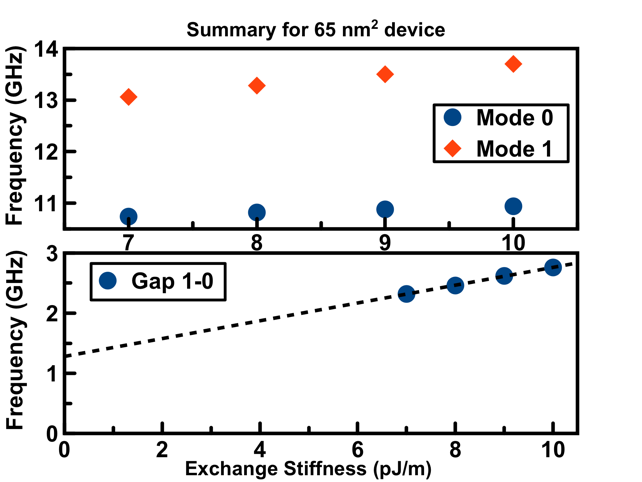
\includegraphics[width=60mm]{fig/2018/sim/65sim}} &
      \addheight{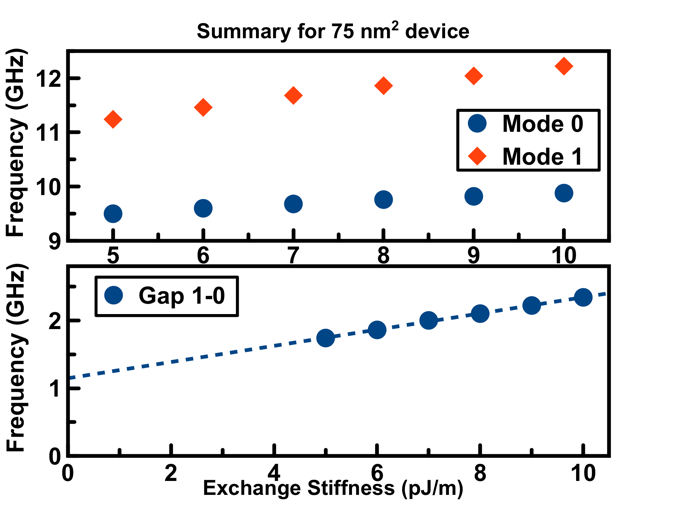
\includegraphics[width=60mm]{fig/2018/sim/75sim}} \\
      \addheight{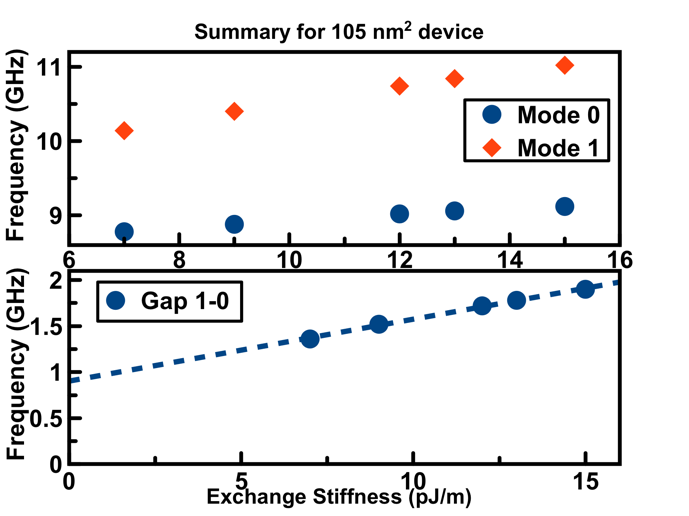
\includegraphics[width=60mm]{fig/2018/sim/105sim}} &
      \addheight{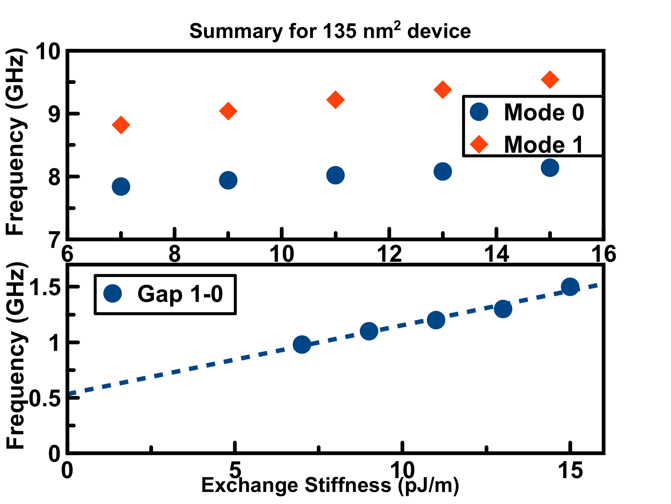
\includegraphics[width=60mm]{fig/2018/sim/135sim}} \\
\end{tabular}
\caption{Circular Device Simulation Summary}
\label{circularsummary}
\end{table}



\begin{figure}[!ht]
  \centering
  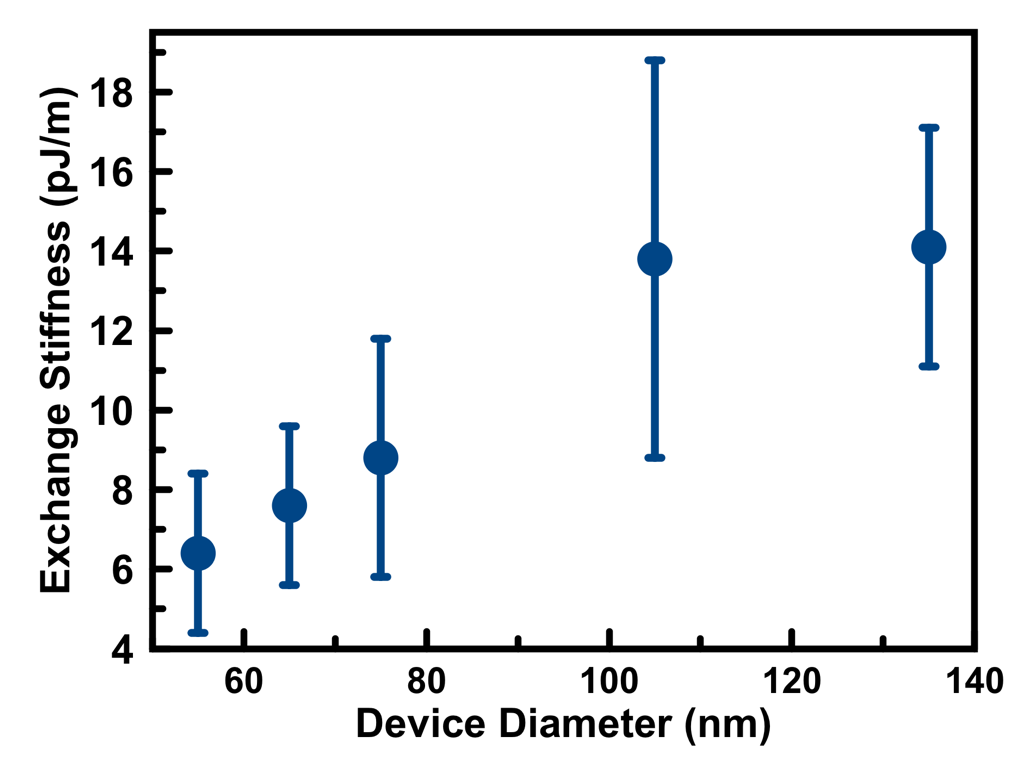
\includegraphics[width=0.6\textwidth]{fig/2018/sim/circular_summary}
   \caption{Circular Device Simulation Summary}
  \label{fig:circularsummary}
\end{figure}


\begin{table}[]
\centering
\begin{tabular}{|l|l|l|l|}
\hline
\textbf{Nominal Device length (nm)} & \textbf{Device Length* (nm)} & \textbf{Aex (pJ/m)} & \textbf{Error (pJ/m)} \\ \hline
\textbf{70} & 55 & 6.4 & 2 \\ \hline
\textbf{80} & 65 & 7.6 & 2 \\ \hline
\textbf{90} & 75 & 8.8 & 3 \\ \hline
\textbf{120} & 105 & 13.8 & 5 \\ \hline
\textbf{150} & 135 & 14.1 & 3 \\ \hline
\end{tabular}
\caption{Circular Device Fit Summary}
\label{cirexsummary}
\end{table}


\begin{figure}[!ht]
  \centering
  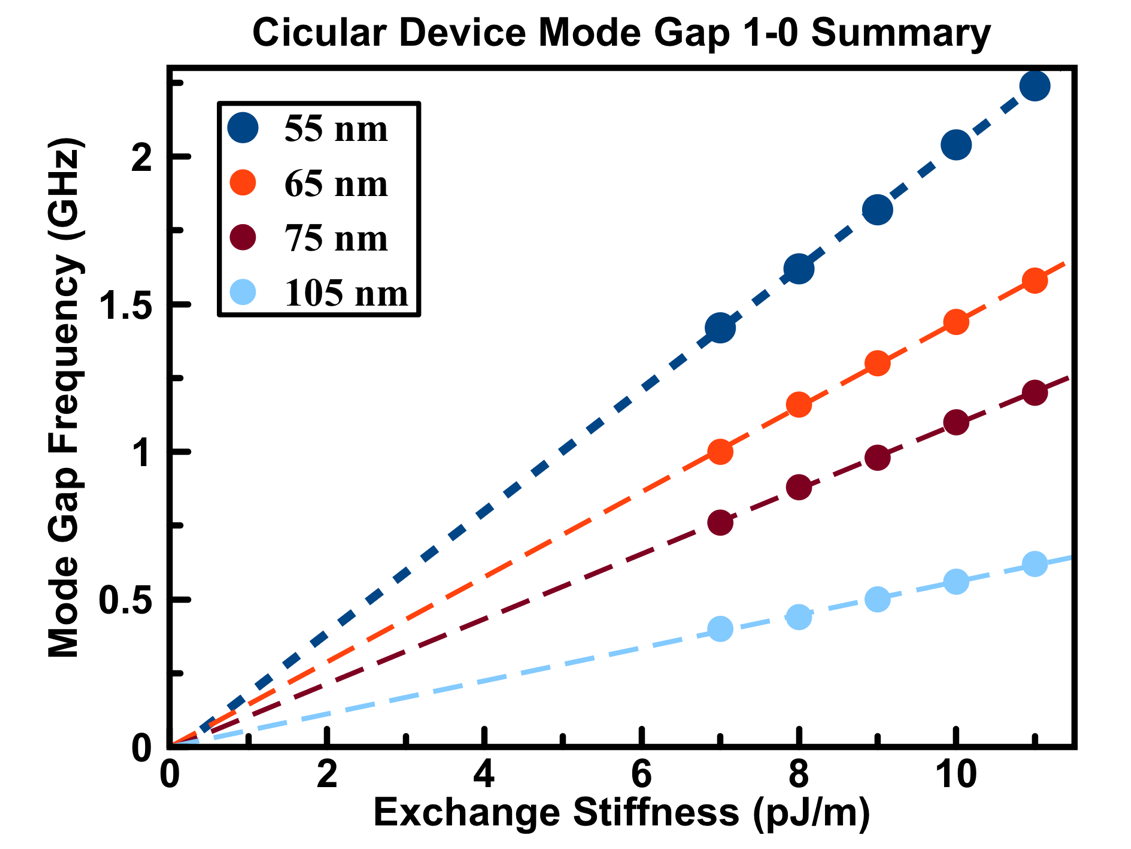
\includegraphics[width=0.6\textwidth]{fig/2018/sim/free_only_circular}
   \caption{Single Free layerCircular Device Simulation Summary}
  \label{fig:freecircularsummary}
\end{figure}



